\subsection{Hypothesis on Time Density}
\label{sec:hypothesis_time_density}

\begin{hypothesis}
\label{hyp:time_density}
Prediction quality of queries are higher on queries where the timestamps are in a temporally dense subset of the training dataset, compared to a sparse subset.
\end{hypothesis}

\begin{figure}[htb]
\centering
\begin{minipage}{0.95\columnwidth}
\centering
\small
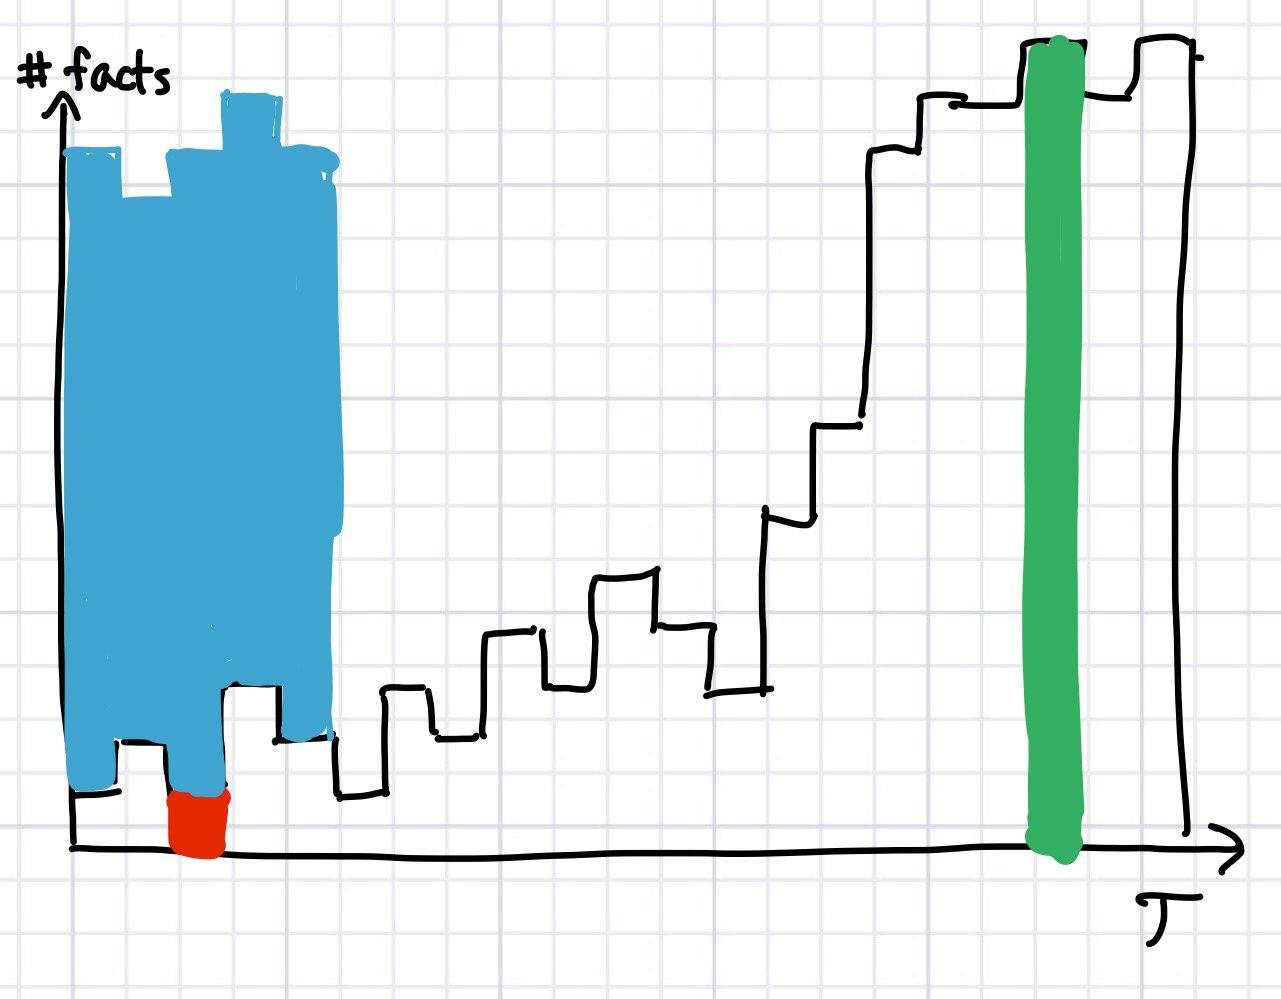
\includegraphics[scale=0.18]{content/hypotheses/figures/time_density.jpg}
\caption{Illustration of \autoref{hyp:time_density}. A dataset with facts sorted by timestamp, timestamp on the Y-axis, fact count on the X-axis.
}
\label{fig:time_density}
\end{minipage}
\end{figure}

This hypothesis is illustrated in \autoref{fig:time_density}. A query from the red bar is expected to have a worse prediction than a query from the green bar because it is in a subset with lower data density. In other words the prediction quality of the same red query would be improved solely by adding correct facts corresponding to the blue extension of the bars.

It will be examined by creating two partitions of approximately same size that contain test facts, one where the temporal density is low and one where it is high. The average prediction rank is then found for each partition. If the dense partition has significantly better MRR score for most of the methods, the hypothesis is deemed true.

More specifically, to evaluate this hypothesis, a function $\mathit{range}$ is defined that denotes which timestamps a time interval contains. The granularity of the timestamps are days for ICEWS14 and years for YAGO and WIKIDATA. It is defined as

\begin{equation}
\mathit{range}(a) = \{ t \in \varT \mid \timebegin{a} \leq t \wedge t < \timeend{a} \}
\end{equation}

\noindent
where $a$ is a time interval.

The $\mathit{range}$ function is then used to define the function $\mathit{num}$, which maps a timespan to a natural number $\varT^2 \rightarrow \N$. This function describes how many facts in $\varG$ that are contained in the timespan. The function is defined as

\begin{equation}
\mathit{num}(a) = \varsum_{(h, r, t, \tau) \in \varG} \I ( \mathit{range}(a) \cup \mathit{range}(\tau) \neq \emptyset )
\end{equation}

\noindent
where $\I$ is a boolean function that evaluates to $1$ if the containing expression is true, $0$ otherwise.

The \nth{25} percentage value $p$ and the \nth{75} percentage value $d$ is found between all temporal granularity timespans $\mathit{num}(\tau)$ for all timespans $\tau$ in the facts of $\varG$. The sparse partition on dataset split $i$ is then defined as

\begin{equation}
T_P = \{ (e_1, r, e_2, \tau) \in \test_i \mid \textit{num}(\tau) < p \}
\end{equation}

\noindent
and the dense partition is defined as 

\begin{equation}
T_D = \{ (e_1, r, e_2, \tau) \in \test_i \mid \textit{num}(\tau) > d \}
\end{equation}

Note that by these definitions the partitions are not continuous.

The MRR score of each method is calculated over the $T_D$ and $T_P$ test sets, on several datasets. If the score is significantly higher in $T_D$, the hypothesis is true, and if the score is significantly higher in $T_P$ the hypothesis is false.

\begin{comment}
foreach fact in dataset
    fact_count_i_timespan(fact) >> array
done
sort(array)
median(array)
\end{comment}